
\chapter{Mengenal Kecerdasan Buatan dan Scikit-Learn}
Buku umum teori lengkap yang digunakan memiliki judul\textit{Artificial intelligence: a modern approach}\cite{russell2016artificial}.
Untuk pratikum sebelum UTS menggunakan buku \textit{Python Artificial Intelligence Projects for Beginners}\cite{eckroth2018python}. Buku pelengkap penunjang penggunaan python menggunakan buku \textit{Python code for Artificial Intelligence: Foundations of Computational Agents}\cite{poole2017python}.
Dengan praktek menggunakan python 3 dan editor anaconda dan library python scikit-learn.
Tujuan pembelajaran pada pertemuan pertama antara lain:
\begin{enumerate}
	\item
	      Mengerti definisi kecerdasan buatan, sejarah kecerdasan buatan, perkembangan dan penggunaan di perusahaan
	\item
	      Memahami cara instalasi dan pemakaian sci-kit learn
	\item
	      Memahami cara penggunaan variabel explorer di spyder
\end{enumerate}
Tugas dengan cara dikumpulkan dengan pull request ke github dengan menggunakan latex pada repo yang dibuat oleh asisten riset.

\section{Teori}
Praktek teori penunjang yang dikerjakan :
\begin{enumerate}
	\item
	      Definisi, Sejarah dan perkembangan Kecerdasan Buatan.
	      \begin{itemize}
		      \item Definisi
		            \par \setlength{\parindent}{5ex}
		            AI (Artificial Intelligence) atau dikenal dengan nama Kecerdasan Buatan merupakan implementasi kecerdasan yang dimiliki manusia pada mesin atau sebuah program sehingga program tersebut dapat berpikir selayaknya seorang manusia.
		            \par Pengetahuan yang digunakan oleh AI merupakan pengetahuan yang berbentuk data yang diinputkan oleh manusia pembuatnya. 	Pada AI terdapat poin penting yang berupa \emph{learning, reasoning,} dan \emph{self correction}. Pada tahap learning, AI dapat 		mengimprovisasi pengetahuannya tanpa bantuan manusia. AI melakukan improvisasi dengan menggunakan data seadanya yang pernah diinputkan oleh manusia. Reasoning merupakan penalaran atau pemberian alasan atau pemecahan oleh AI dengan menggunakan pengetahuan yang dimilikinya. Selain itu, self correction adalah kemampuan untuk memperbaiki keputusan yang salah ambil dan perupakan proses belajar AI melalui pengamatan sekitarnya.
		            \par AI merupakan kecerdasan buatan yang didalamnya terdapat faktor \emph{Acting Humanly} (Tindakan AI yang selayaknya manusia), \emph{Thinking Humanly} (Pola pikir selayaknya manusia), \emph{Think Rationally }(Berpikir Rasional selayaknya manusia), dan \emph{Act Rationally} (Bertindak rasional selayaknya manusia).

		      \item Sejarah dan Perkembangan
	      \end{itemize}


	\item
	      Definisi supervised learning, klasifikasi, regresi dan unsupervised learning. Data set, training set dan testing set.
	      \begin{itemize}

		      \item Supervised Learning dan Unsupervised Learning
		            \par \setlength{\parindent}{5ex}
		            Supervised Learning merupakan Algoritma yang digunakan dalam sebuah data science. Supervised learning digunakan pada algoritma kecerdasan buatan dan digunakan untuk membuat prediksi atau klasifikasi. Supervised learning berarti kita memasukan sebuah pengetahuan baru kedalam otak AI.
		            \par Sedangkan pada \emph{Unsupervised Learning} berarti kita tidak perlu memasukan pengetahuan yang baru ke dalam otak AI. Hal tersebut karena pada algoritma \emph{unsupervised learning} ini, AI akan improvisasi tanpa harus dilatih terlebih dahulu.

		      \item Klasifikasi dan Regresi
		            \par \setlength{\parindent}{5ex}
		            Klasifikasi merupakan teknik untuk melakukan klasifikasi atau pengelompokan atau pengkategorian terhadap item - item yang belum berlabel ke dalam sebuah set kelas diskrit.
		            \par Regresi merupakan sebuah teknik untuk melakukan itentifikasi hubungan atau relasi antar variabel (dua atau lebih). Regresi digunakan untuk menemukan sebuah fungsi yang memodelkan data dengan meminimalisir error atau selisih antara nilai prediksi dan nilai sebenernya.

		      \item Dataset, Training Set dan Testing Set
		            \par \setlength{\parindent}{5ex}
		            \emph{Dataset} merupakan himpunan data atau kumpulan data yang dikumpulkan dari data data yang terdahulu (data dari masa lampau). Kemudian data tersebut diolah menjadi sebuah informasi untuk digunakan pada Data Mining atau Kecerdasan buatan.
		            \par \emph{Training Set} merupakan bagian dari dataset yang sudah dilatih untuk membuat prediksi atau menjalakan fungsi dari algoritma pada \emph{Machine Learning}.
		            \par \emph{Test Set} merupakan bagian dari data set yang digunakan untuk melihat keakuratan dan performa dari dataset tersebut.

	      \end{itemize}
\end{enumerate}

\section{Instalasi}
Membuka https://scikit-learn.org/stable/tutorial/basic/tutorial.html. Dengan menggunakan bahasa yang mudah dimengerti dan bebas plagiat.
Dan wajib skrinsut dari komputer sendiri.
\begin{enumerate}
	\item
	      Instalasi library scikit dari anaconda, mencoba kompilasi dan uji coba ambil contoh kode dan lihat variabel explorer[hari ke 1](10)\\
	      \begin{itemize}
		      \item
		            Instalasi Scikit-Learn\\
		            Menggunakan perintah
		            \begin{verbatim}
					pip install scikit-learn
					\end{verbatim}
		            \begin{figure}[H]
			            \centering
			            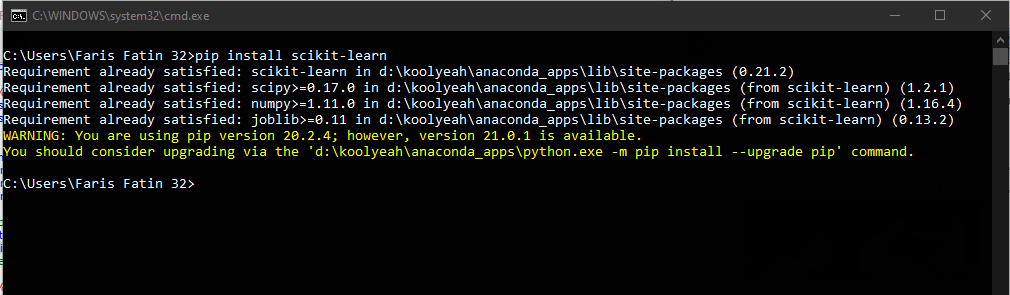
\includegraphics[scale=0.5]{c1-1}
			            \caption{installasi Scikit-Learn}
		            \end{figure}


		      \item
		            Uji Coba kode dan Melihat Variable Explorer\\
		            \lstinputlisting[language=python]{./snippets/Chapter1/install.py}
		            Variabel Explorer:
		            \begin{figure}[H]
			            \centering
			            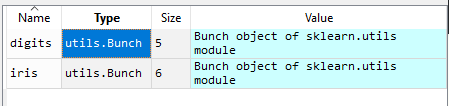
\includegraphics[scale=1]{c1-2}
			            \caption{Variabel Explorer}
		            \end{figure}
		            \begin{itemize}
			            \item
			                  Variabel digits:
			                  \begin{figure}[H]
				                  \centering
				                  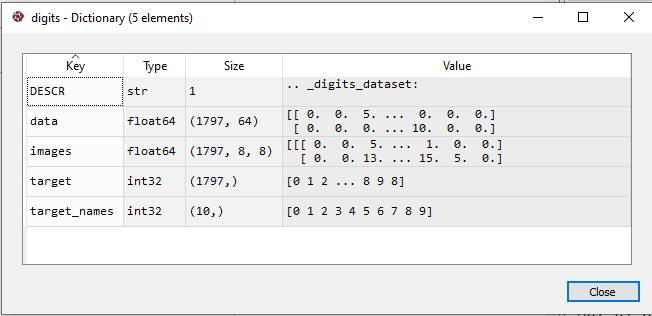
\includegraphics[scale=0.7]{c1-3}
				                  \caption{Variabel digits}
			                  \end{figure}
			            \item
			                  Variabel iris:
			                  \begin{figure}[H]
				                  \centering
				                  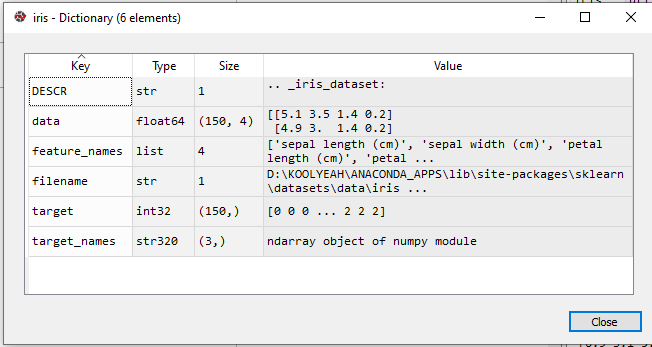
\includegraphics[scale=0.7]{c1-4}
				                  \caption{Variabel iris}
			                  \end{figure}
		            \end{itemize}
	      \end{itemize}


	\item
	      Loading an example Dataset
	      \par \setlength{\parindent}{5ex}
	      Bagian ini adalah percobaan memuat kumpulan data. Library scikit-learn sendiri memiliki tiga buah dataset. Dataset iris digunakan untuk contoh, dataset digits digunakan untuk klasifikasi, dan dataset diabetes untuk regresi.
	      \lstinputlisting[language=python, caption=Loading an Example Datasets, firstline=1, lastline=7]{./snippets/Chapter1/LoadingAnExampleData.py}
	\item
	      Mencoba Learning and predicting
	      \par \setlength{\parindent}{5ex}
	      Bagian ini merupakan bagian untuk belajar dan melakukan prediksi dari sebuah gambar. Gambar yang akan diprediksi merupakan gambar digit sehingga dataset yang digunakan adalah dataset digits
	      \lstinputlisting[language=python, firstline=10, lastline=13, caption=Learning and predicting]{./snippets/Chapter1/LoadingAnExampleData.py}
	\item
	      Mencoba Model persistence
	      \par \setlength{\parindent}{5ex}
	      Model persistence merupakan model yang digunakan untuk menyimpan data sehingga ketika program akan digunakan kembali, program tidak perlu dilatih ulang dari nol. Model ini dapat disimpan dengan menggunakan pickles atau joblib
	      \lstinputlisting[language=python, caption=Learning and predicting]{./snippets/Chapter1/modelPersistence.py}
	\item
	      Mencoba Conventions
	      \par \setlength{\parindent}{5ex}
	      Conventions adalah
	      \lstinputlisting[language=python, caption=Learning and predicting]{./snippets/Chapter1/conventions.py}
\end{enumerate}


\section{Penanganan Error}
Dari percobaan yang dilakukan di atas, apabila mendapatkan error maka:

\begin{enumerate}
	\item
	      skrinsut error[hari ke 2](10)
	\item
	      Tuliskan kode eror dan jenis errornya [hari ke 2](10)
	\item
	      Solusi pemecahan masalah error tersebut[hari ke 2](10)

\end{enumerate}

